\documentclass[assd_tp2_main.tex]{subfiles}

\begin{document}

\section{Programa principal}
Se desarrolló un software para procesar archivos midis mediante las funciones de síntesis de instrumentos. Se utilizaron distintas librerias de python, entre ellas mido (para leer los archivos midi) y tkinter (para poder realizar una interfaz gráfica)

Los resultados fueron exitosos; se logró desarollar una interfaz gráfica funcional que brindó la capacidad para seleccionar los instrumentos, el volumen de los canales, mostrar el espectograma de la canción resultante.


\begin{figure}[H]
\centering
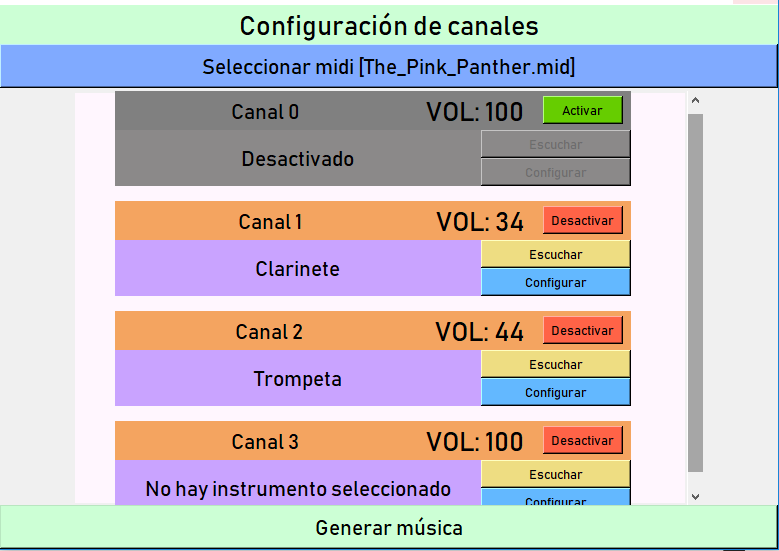
\includegraphics[width=1\linewidth]{graficos/gui.png}
\caption{Ejemplo funcionamiento GUI}

\end{figure}

Se adjunta el codigo fuente en la entrega de este práctico.
\end{document}